\documentclass{article}
\usepackage{v-equation}
\vgeometry

\begin{document}
\def\gdrive{https://drive.google.com/drive/folders/1ajNP86BKmDGvWcw2mtQQ9XMr1iYNT4Gj?usp=share_link}

\vtitle[Coulomb’s Law in a dielectric]
\begin{center}
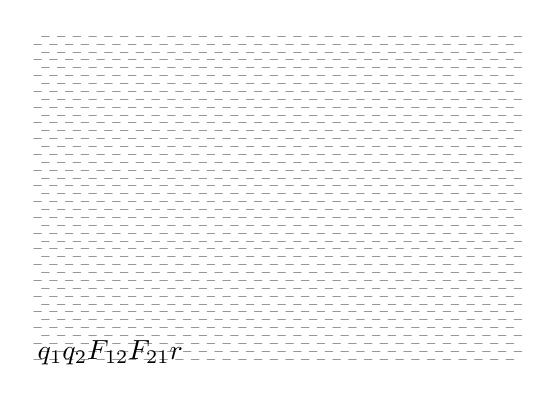
\begin{tikzpicture}
\begin{scope}
\foreach \s in {0, 0.1}{
	\foreach \x in {0,0.2,..., 6}{
		\foreach \y in {0, 0.2,..., 4}{
			\node at (\x+\s, \y+\s)[scale=0.5, opacity=0.75] {$-$};
		}
	}
}
\end{scope}
\tzcoor*(1,2)(Q1){$q_1$}[bl](5pt)
\tzcoor*(5,2)(Q2){$q_2$}[br](5pt)
\tzline+[->] (Q1)(-1.5, 0){$F_{12}$}[l]
\tzline+[->] (Q2)(1.5, 0){$F_{21}$}[r]
\tzline[|<->|]<0, -0.5>(Q1)(Q2){$r$}[mb]
\end{tikzpicture}
\end{center}
\vspace*{\fill}
\begin{align*}
\varepsilon_0 &= \textit{permittivity of free space}\\
\varepsilon &= \textit{permittivity of medium}\\
K &= \textit{dielectric constant}\\
\varepsilon &= K\varepsilon_0  \\
F_e &= \textit{force in vacuum} \\
F'_e &= \textit{force in the medium} 
\end{align*}
\vspace*{\fill}

\pagebreak

\addtolength{\jot}{3ex}
\begin{align*}
F_e &= \dfrac{1}{4\pi\varepsilon_0} \cdot \dfrac{q_1q_2}{r^2}\\
F'_e &= \dfrac{1}{4\pi\varepsilon} \cdot \dfrac{q_1q_2}{r^2}\\
\dfrac{F_e}{F'_e} &= \dfrac{\varepsilon}{\varepsilon_0} \\
\dfrac{F_e}{F'_e} &= \dfrac{K\varepsilon_0}{\varepsilon_0} \\
\Aboxed{F'_e &= \dfrac{F_e}{K}}
\end{align*}
\pagebreak

\vspace*{\fill}
\begin{center}
    \fbox{\qrcode[height=2cm]{\gdrive}}
\end{center}
\vspace*{\fill}
\end{document}
